% Settings for the default beamer theme
\documentclass[english, aspectratio=169]{beamer}
\usepackage[T1]{fontenc}
\usepackage[utf8]{inputenc}
\usepackage{tabularx}
\usepackage{babel}
\usepackage[ruled,vlined]{algorithm2e}
\SetAlgorithmName{Algoritmus}{algoritmus}{List of Algorithms}
\setcounter{secnumdepth}{3}
\setcounter{tocdepth}{3}

\makeatletter

\newcommand\makebeamertitle{\frame{\maketitle}}

% (ERT) argument for the TOC
\AtBeginDocument{%
  \let\origtableofcontents=\tableofcontents
  \def\tableofcontents{\@ifnextchar[{\origtableofcontents}{\gobbletableofcontents}}
  \def\gobbletableofcontents#1{\origtableofcontents}
}

% Theme settings
\usetheme{Frankfurt}
\usecolortheme{default}
\usefonttheme[onlymath]{serif}

% Template settings
\setbeamertemplate{navigation symbols}{}
\setbeamertemplate{blocks}[rounded][shadow=false]
\setbeamertemplate{title page}[default][colsep=-4bp, rounded=true, shadow=false]
\makeatother

% Define a custom darker red color
\definecolor{DarkerRed}{RGB}{139,0,0} % Adjust the RGB values as needed

% Use the newly defined color in Beamer theme elements
\setbeamercolor{structure}{fg=DarkerRed} % Changes basic structural elements to Darker Red
\setbeamercolor{title in head/foot}{bg=DarkerRed} % Changes the title in header/footer to Darker Red


\begin{document}

% Title page
\section{Bevezetés}
\title[]{Üzleti Elemzések Módszertana}
\subtitle{2. Előadás: Osztályozás}
\author[Kuknyó Dániel]{Kuknyó Dániel\\Budapesti Gazdasági Egyetem}
\date{2023/24\\2.félév}
\makebeamertitle

% Table of contents slide
\begin{frame}
\tableofcontents{}
\end{frame}

% Table of contents of the current section
\begin{frame}
\tableofcontents[currentsection]
\end{frame}

\begin{frame}{A determinisztikus szemléletmód}
\begin{columns}
\begin{column}{.5\textwidth}
A hagyományos szoftverfejlesztési folyamatmodell eljárása:
\begin{enumerate}
	\item Az adott jelenség megfigyelése és adatok rögzítése
	\item A megfigyelésekre olyan szabályok kidolgozása, amelyek jól leírják azt
	\item A létrejött szabályrendszer kiértékelése
	\item Rendszer fejlesztése a hibák alapján
	\item Iteráció
\end{enumerate}
\end{column}
\begin{column}{.5\textwidth}
\begin{center}
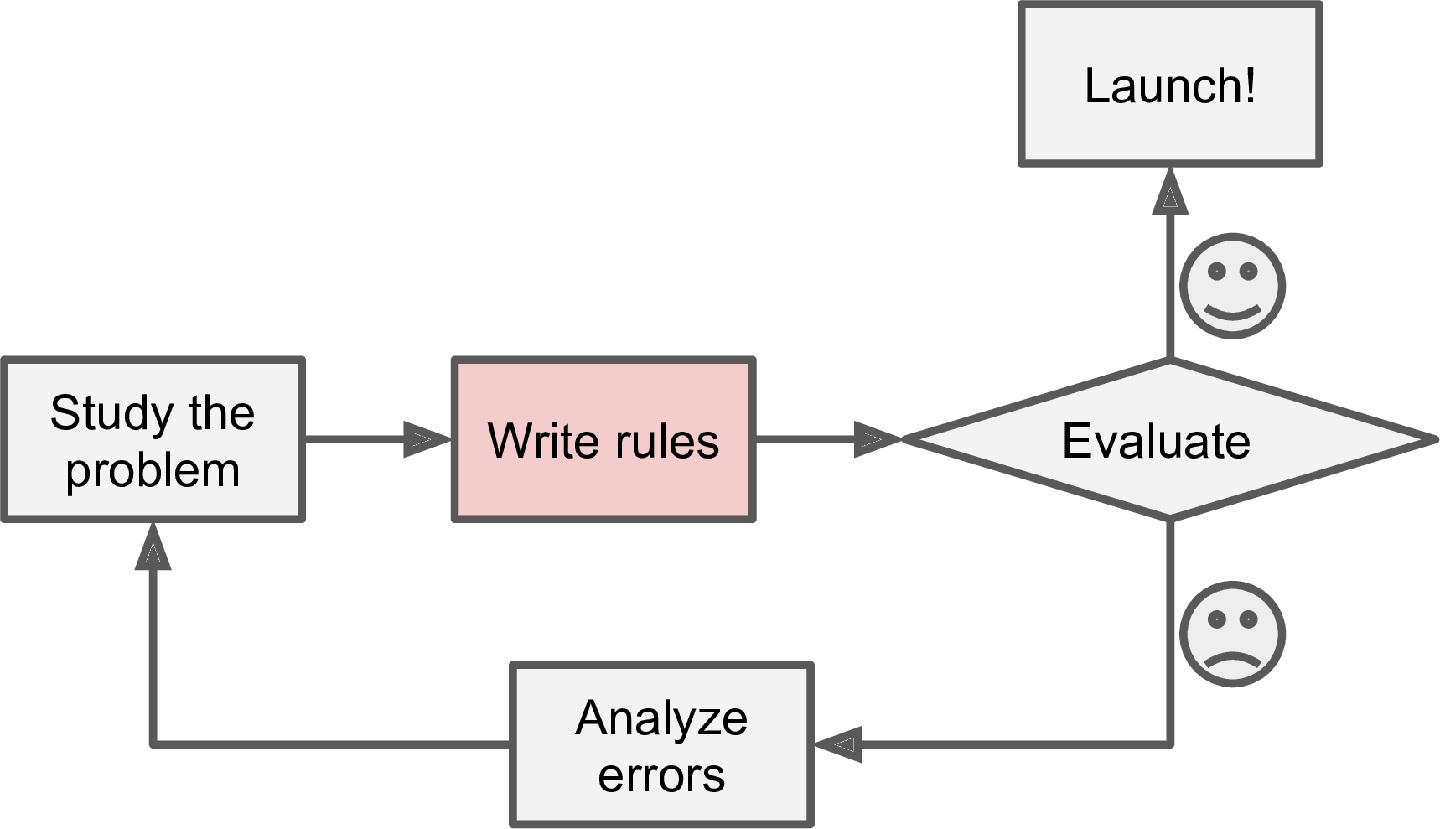
\includegraphics[width=7cm, height=7cm, keepaspectratio]{images/osztalyozas_1.png}
\end{center}
\end{column}
\end{columns}
\end{frame}

\begin{frame}{A gépi tanulás szemléletmód}
\begin{columns}
\begin{column}{.5\textwidth}
A gépi tanulás szemléletének folyamatmodellje:
\begin{enumerate}
	\item Adott jelenség megfigyelése és adatok rögzítése
	\item Gépi tanulási modell tanítása az adatokon a szakterületi tudás segítségével
	\item Modell kiértékelése
	\item Hibák elemzése és kiértékelése
	\item Iteráció
\end{enumerate}
\end{column}
\begin{column}{.5\textwidth}
\begin{center}
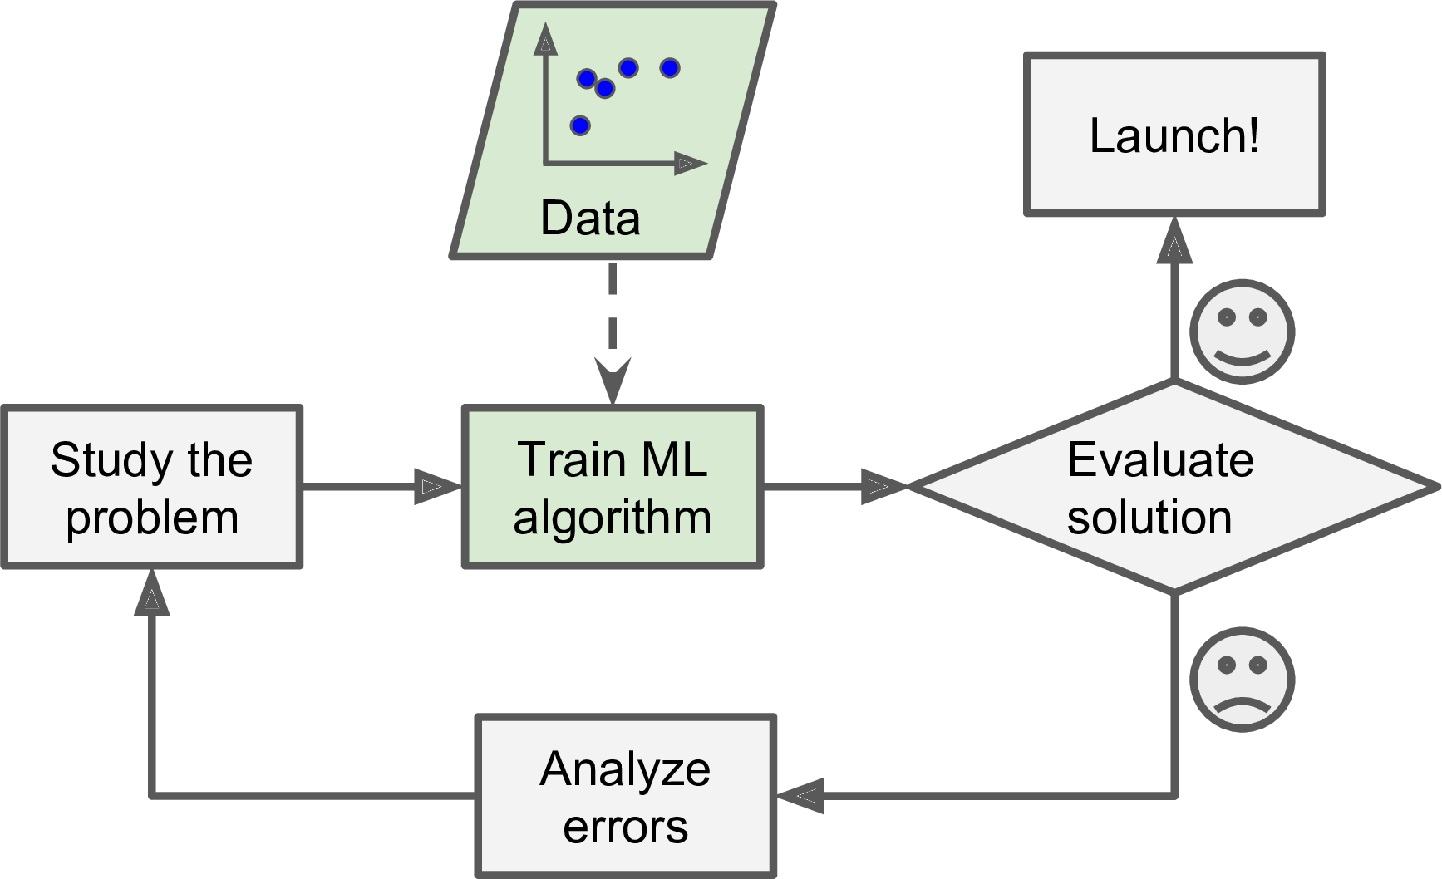
\includegraphics[width=7cm, height=7cm, keepaspectratio]{images/osztalyozas_2.png}
\end{center}
\end{column}
\end{columns}
\end{frame}

\begin{frame}{Tanítás automatizálása adatalapúan}
\begin{columns}
\begin{column}{.5\textwidth}
Az gépi tanuló modellek tanítása és kiértékelése hosszú távon egy iteratív folyamat már létező keretrendszerekkel, mint az MLOps. Ennek számos területen vannak előnyei:
\begin{itemize}
	\item Adaptáció az új adatokhoz
	\item Javuló modell teljesítmény
	\item Hibák és problémák azonosítása
	\item Új technológiai fejlődés integrálása
	\item Skálázhatóság és rugalmasság
	\item Szakterületi következtetések az elemzések által
\end{itemize}
\end{column}
\begin{column}{.5\textwidth}
\begin{center}
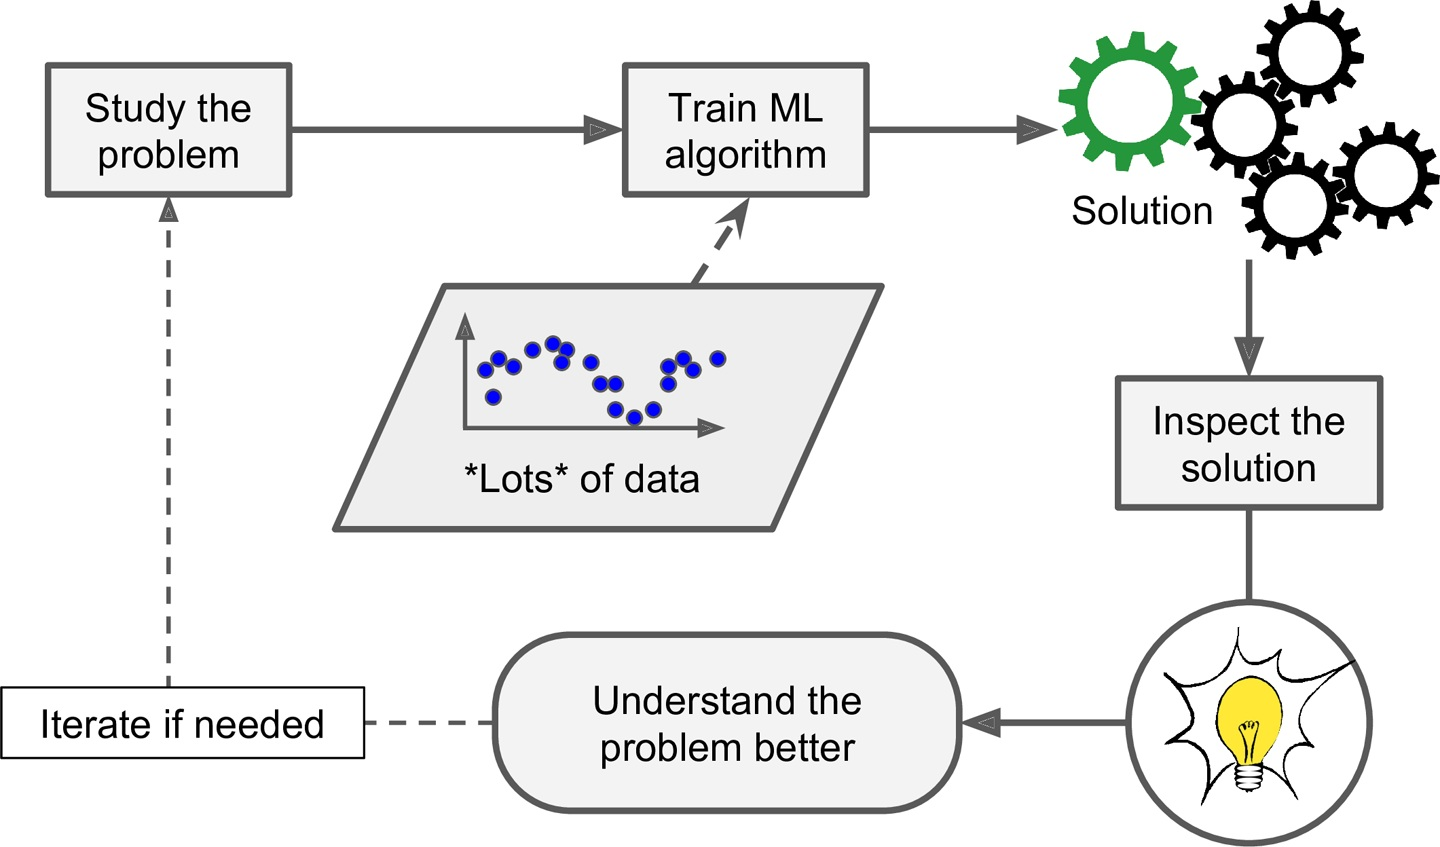
\includegraphics[width=7cm, height=7cm, keepaspectratio]{images/osztalyozas_3.png}
\end{center}
\end{column}
\end{columns}
\end{frame}

\section{Osztályozás}

\begin{frame}
\tableofcontents[currentsection]
\end{frame}

\begin{frame}{Osztályozás}
\begin{columns}
\begin{column}{.5\textwidth}
\begin{block}{Osztályozás}
Az osztályozás a felügyelt gépi tanulás egyik alapvető feladata, amelynek célja, hogy megtanuljon egy modellt vagy szabályrendszert egy adott bemeneti adat alapján \textbf{annak besorolására előre meghatározott kategóriákba vagy csoportokba}. 
\end{block}
\end{column}
\begin{column}{.5\textwidth}
\begin{center}
\includegraphics[width=7cm, height=7cm, keepaspectratio]{}
\end{center}
\end{column}
\end{columns}
\end{frame}

\end{document}





















